\documentclass[a4paper, 10pt, notitlepage]{article}

\usepackage{amsfonts} % if you want blackboard bold symbols e.g. for real numbers
\usepackage{graphicx} % if you want to include jpeg or pdf pictures
\usepackage[margin=1.25in]{geometry}
\usepackage{comment}

\setlength{\parskip}{\baselineskip}%
\setlength{\parindent}{0pt}%

\title{6.830 Project: Partitioned database with deadlock detection}
\author{Benjamin Mattocks, Wenting Zheng}
\date{May 16, 2013} % change this

\begin{document}

%%%%%%%%%% PRELIMINARY MATERIAL %%%%%%%%%%
\maketitle
\thispagestyle{empty}
\newpage

%%%%%%%%%% MAIN TEXT STARTS HERE %%%%%%%%%%

\section{Introduction}

Although distributed databases have been around for a while, and many have been commercialized, there are still many
interesting problems to be solved in this area. Our 6.830 project aims to implement a simple distributed database
and explore some of these problems.

One of the problems we aim to tackle is data partitioning. Although some smaller distributed data may decide to replicate
data across all of the machines, this will not be scalable in the long run, as the amount of data in the database
increases. Therefore, {\em some} kind of data partitioning scheme is needed. Partitioning often brings related problems, such
as hotspots (where ) and . Our project aims to explore workload-based re-partitioning to increase throughput.

Another problem that is present in distributed databases is deadlock detection. Deadlocks are usually rare, but it is necessary
to be able to detect them efficiently so that the database can continue to handle transactions. Distributed deadlock detection
is quite hard. Since deadlock can only be detected in a global way, this makes it very easy to falsely detect deadlocks and
incorrectly abort transactions.


\section{Previous Work}

\subsection{Database partitioning}
Ghandeharizadeh and DeWitt [2] introduce a hybrid-range partitioning strategy, which optimizes partitioning by the types of queries and leading to a higher level of parallelism and load-balancing. It attempts to reduce load and provide load balancing.

Yu et al. [5] introduce a partition and replicate strategy for a database which does not necessarily require a large number of partitions. This algorithm works well where the number of number of relations is small and the network is uniform in terms of processing speed.

Liu and Chen [3] describe a hash partitioning strategy for distributed query processing, expanding on the work of Yu et al. The strategy is described for relation partitioning where relations are unfragmented and replicated in a shared-nothing environment. They use a heuristic to determine which data should be partitioned to which site.

\subsection{Deadlock detection}
Chandy et al. [1] describe a distributed probing system in which a deadlock can be detected when a probe reaches its origin by following the WFG. A transaction waiting for a lock sends a probe with its transaction ID to any transactions it is waiting upon and other waiting transactions propagate this probe if they are also waiting.

Mitchell and Merritt [4] propose a probe-based deadlock detection algorithm which traverses the edges in the WFG backwards. Each transaction contains a public and private label, and the messages are propagated by the order label.

There are also numerous other techniques that make use of constructing global data at a single point and determining deadlocks based on transaction locking information. However, these are prone to using out of date information in distributed settings.


\section{Data storage}

\subsection{Design}
Our distributed database implements a key-value storage system with transaction support. Unlike a pure key-value storage, however,
it keeps the concept of tables. The tables are organized as {\em (primary key, record value)}.
The interface for accessing data contains the two operations: \texttt{write(table\_name, key, value)} and \texttt{read(table\_name, key)}.
Thus, the data storage supports atomic groups of reads and writes.

\subsection{Implementation}
The implementation of the data storage is based on hash tables. Each partition contains a hash table storing the table names and a list
of key-values associated with that table. Since the hashing is done on the primary keys, a partition needs to store smaller key-value
stores that correspond to different tables. 

\section{Two Phase Locking and Two Phase Commit}

\subsection{Background}
The database needs to be able to handle distributed transactions. A commit should make sure the database shows all of a transaction's
changes, and an abort should make sure none of the changes are made. There can be no inconsistent state in here. Therefore, two phase
locking is there to make sure that the read values are read correctly, and that the write values are written correctly and not
overwritten by another transaction by the time commit happens.

On the other hand, two phase commit guarantees commits and aborts to be consistent across all machines in case of failures. The 
two phase commit protocol selects a coordinator for each transaction, and the coordinator ultimately decides whether that particular
transaction will commit and abort after gathering information from all of its cohorts (the other servers involved in the transaction).

\subsection{Implementation}

Each server keeps its own lock table. The lock table provides both read locks and write locks. For this implementation, we only provide
record-level locking. Transactions are only able to lock specific records. However, in the future we plan on supporting hierarchical
locking. 

The implementation for two-phase locking is strong strict two phase locking. Both read and write locks are held until the transaction
commits or aborts. This is the implementation because the code is written in such a way that the transaction's read and write values
can be requested multiple times until commit happens. Therefore, the end of phase 2 is right before commit happens, and SS2PL is the
correct implementation to ensure atomic transactions.

Two phase commit requires a coordinator for each transaction. Every transaction selects a coordinator the moment
it starts. Since every transaction is routed to a server to start, that server is the coordinator. The coordinator then looks
into its partition table for a list of all the cohorts it needs to contact. When commit or abort happens, the coordinator
contacts the necessary servers to get a list of votes, and 2PC proceeds as normal.

Our 2PC protocol is limited because the recovery process has not been written yet. Other than the logging and the recovery
process, the basic 2PC algorithm is implemented. In the future we would like to look into presumed commit or presumed abort.

\section{Partitioning}

\subsection{Background}

Some kind of partitioning scheme is required in a distributed database. There are several ways of approaching
this topic. The two most popular methods are hashing and range partitioning.

Range partitioning seems attractive when transactions tend to access records that are close to each other
in a table. This often happens when transactions perform a large number of range scans. However, range partitioning
requires some knowledge of the schema, and is often difficult to implement. It is also easy to get hotspots for
range partitioning.

On the other hand, hashing tends to randomize keys. This partitioning scheme is not so great for range scans
since it will most likely distribute similar keys far away from each other. However, hashing does have its advantages.
It is very easy to implement, which is the main reason why so many industrial implementations use hashing as its
partitioning method. It is also easy to scale up as the number of keys increases. 

For this project, we decided to implement a hashing-based partitioning scheme, with an adjustable number of partitions.
Based on the workload and the machine limit, the user can choose to either to have fine-grained partitioning or
coarse-grained partitioning.

\subsection{Dynamic Re-Partitioning}

Dynamic re-partitioning are often used in large distributed storage systems for a number of reasons. The main reason is
to partition the data in such a way so that transactions are run with maximum efficiency. This often leads to the following:

1. Large transactions are run in parallel. For example, transactions that modify or read a large number of data sets
can be executed quite fast if most of the partitions it needs to read/modify are done on separate machines in parallel.

2. Small transactions are run locally. If a transaction is very small, then it is too costly to run a distributed transaction,
which would involve sending a lot of network messages. 

A good and efficient partitioning scheme is very difficult design. The two previous points are somewhat contradictory with each
other. Thus, in a generalized database, one would have to carefully collect transaction profiles in order to develop a good
re-partitioning.

In our database we try to reduce the number of distributed transactions executed. If we have a set of small transactions that are 
run repeatedly, modifying and reading a small number of records, then it is better to reduce the number of distributed transactions 
as much as possible. The main idea of our partitioning scheme is to hash the primary keys, but finely partition the data set enough 
so that we can counter the randomness of hashing. 

Partitions are related to each other based on how often they are run together in the same transaction. For each partition pair, we
keep an {\em affinity factor} (or {\em AF}) that shows how closely related two partitions are with each other. The {\em AF} are
increased only at the coordinator of a transaction. The reconfiguration plan is constructed based on the {\em AF} information

\subsection{Implementation}

Each server keeps track of two tables. The first table is a partition table. The partition table stores mappings of partition number
to a server address. The partition table also has a single version number. The second table is an {\em AF} table.
The {\em AF} table keeps a list of pairs of partitions, and a number indicating the relationship between these two partitions.
Every time a successful commit happens, the coordinator of that transaction increases the {\em AF} number for each pair of participating
partitions. 

There is a server designated as the reconfiguration master. Currently, the master's identity does not change. The master server
periodically sends out requests for {\em AF} information. Once the master server receives all of the {\em AF} information, it
constructs a weighted graph of all partitions in the server pool. The heavier the edge, the closer the partitions should be 
put next to each other. 

The master then runs an algorithm to produce a reconfiguration plan. The algorithm is very simple. It simply takes the heaviest
edge in the graph and brings the two partitions together on the same machine, if they are not already on the same machine.
If a partition is moved from machine A to machine B, another partition must be moved from machine B to machine A. Note that the
assumption here is that all partitions are almost equally involved in the workload. 

Once the master decides on a plan, it sends the plan to all of the workers. The master and the workers then start the reconfiguration
algorithm. The server first changes its reconfiguration state to {\em CHANGE}, and waits for all current transactions to commit
or abort. While in this state, the server does not receive any more transactions.
If a server does not have a local transaction started, or all of its transactions have been finished, the server goes
to the next step, where it looks at the reconfiguration plan and sends all of the partitions that need to be sent. Because of the 
algorithm, most of the servers will not need to send or receive any partition. After this step is done, the server updates its
partition table and increases the table's version number. It then changes the reconfiguration state to {\em READ}, and is ready
to handle more transactions.

When there is a reconfiguration happening, transactions can come in simultaneously. It is very important to make sure that the effects
of the transactions are seen by all partitions. In our database we use a very conservative approach. Transactions that involve servers
that are currently reconfiguring are aborted. Transactions that involve servers with different partition tables are also aborted.


\section{Deadlock detection}

\subsection{Deadlocks}
A deadlock occurs when two or more process are requesting locks to items being held by other processes. More formally, it can be modeled as a Wait-For-Graph, in which a resource has a directed edge to another resource which holds a lock to an item the first resource requests. If there is a cycle in this graph, a deadlock is present.

In a distributed system, deadlock detection has been the subject of numerous studies because the distributed nature adds some complexity to the system, so certain deadlock detection algorithms might not work in a distributed environment. Distributed deadlock detection can be done with the use of centralized servers which keep track of the state of a distributed system, or they can be performed in a completely distributed manner. One problem that could occur with deadlock detection is that deadlocks might be falsely detected, which can negatively impact a system's performance. Some specific causes of this would be message delays across servers or using stale information in the WFG computed at a central server.

\subsection{Implementation}
We decided to implement a fully distributed algorithm, proposed by Chandy, Misra, and Haas. This is an edge-chasing algorithm, which passes probe messages between resources directly. It is based on the AND model of deadlock detection, which sends a probe to all other transactions it depends on which hold a lock to all of its resources. The main idea is that the origin of the first probe knows that a deadlock is present if that probe message is received by the origin a second time. If a process is also waiting for a lock and receives a probe, it sends the probe message along to any other processes which hold locks to resources it is requesting. It retains the origin in its state so the origin will know that it sent that probe if the probe reappears there.

To implement this, we ran a new thread for each transaction (separate from the transaction's main thread) on our distributed database which specifically handles these deadlock probes, independently of the main thread. This allows a worker to detect a deadlock while a specific lock is being requested. If a deadlock thread detects that a probe message it receives was initiated by itself, then it reports a deadlock to the worker thread and aborts the transaction. Specifically, the deadlock detection thread sets a flag in the transaction's main thread, which then triggers an abort message to be sent by our RPC protocol to itself.

\subsection{Test scenario}
%[figure - simple probe messages, originating at W1]
\begin{figure}[h!]

  \centering
    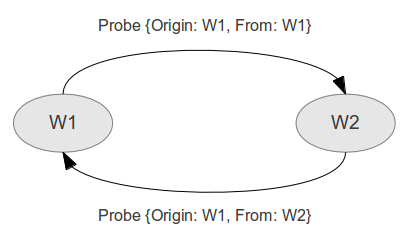
\includegraphics[scale=0.9]{deadlock-message.png}
  \caption{Probe message being propagated in network. The probe originating at W1 is sent to W2, and W2 sends the probe back to W1. W1 detects a deadlock upon arrival of the probe coming from W2.}
\end{figure}

We tested the simple case of two workers in separate threads wanting to obtain a lock held by the other concurrently. Suppose a worker W1 holds a lock on A and is attempting to get a lock on B. If a worker is attempting to lock a resource but cannot obtain the lock, a new probe message is sent to every other resource that holds a lock the worker requests. Suppose W2 holds the lock to B and wants the lock to A. If W1 first sends a probe message to W2, then W2 will send a probe message to W1 because W1 holds the lock to A, which W2 wants. W1 will receive this message and note that this message originated there, so it declares a deadlock and aborts itself.


\section{Analysis and Evaluation}

\subsection{Reconfiguration Evaluation}

For the reconfiguration evaluation, tests were run to compare the performance of the database with and without reconfiguration.
Since we do not have multiple machines available, the reconfiguration tests are run on a single machine. Each virtual server
consists of one thread for accepting RPC messages, one thread for reconfiguration, and one thread for spawning worker
threads to handle transactions.

The tests are run with a variable number of partitions. The range of the keys are from 0 to 4000. The partitions are uniform in that the number
of keys in each partition is roughly the same. The number of partitions are distributed evenly on the virtual servers.
There are four threads running that make requests to the database. The four threads each
represents one type of transaction. The transaction randomly reads 5 to 10 records, and randomly writes 5 to 10 records.
The range of each transaction varies with each test.

Figure 2 and 3 are the data plot for the first test. The number of servers is scaled from 2 to 6. I only
limited it to 6 virtual servers because we see a significant performance reduction with 8 servers due to over-using the number
of cores, thus causing interference between the threads. The four transactions each access 1/4 of the database. The test is 
set up so that deadlock detection does not have to interfere. 

\begin{figure}[h!]

  \centering
    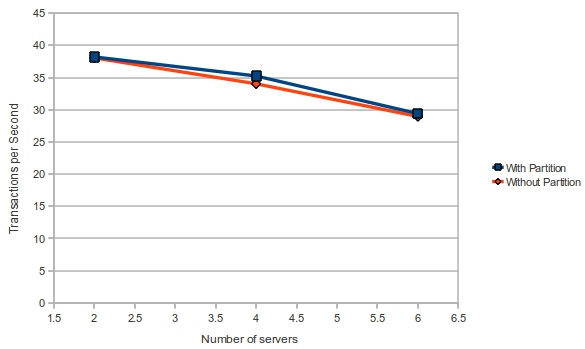
\includegraphics[scale=0.7]{peval1.png}
  \caption{Partition Test 1 -- 20 partitions}
\end{figure}

\begin{figure}[h!]

  \centering
    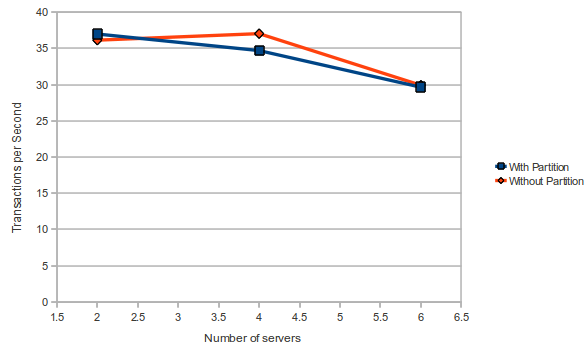
\includegraphics[scale=0.7]{peval2.png}
  \caption{Partition Test 1 -- 80 partitions}
\end{figure}

As we can see, the partitioning did not cause a significant performance increase or decrease. Performance increase is not expected to be seen because
the set of transactions access a random set of records from a rather large range of keys. Performance decrease is seen a little bit
in figure 3, most likely due to the fact that because there are more partitions, the partitioning algorithm is moving partitions
around, thus creating overhead.

The second test was run with four transactions accessing a smaller range of keys. Figure 4 and 5 show the results.

\begin{figure}[h!]

  \centering
    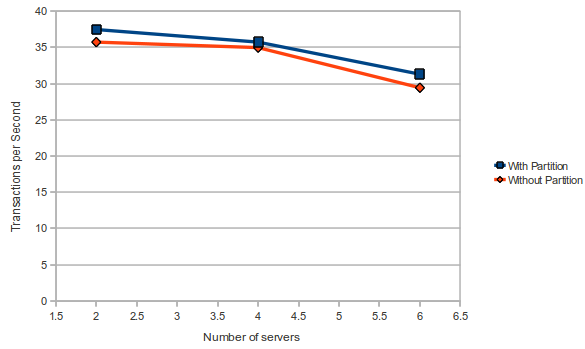
\includegraphics[scale=0.7]{peval3.png}
  \caption{Partition Test 2 -- 20 partitions}
\end{figure}

\begin{figure}[h!]

  \centering
    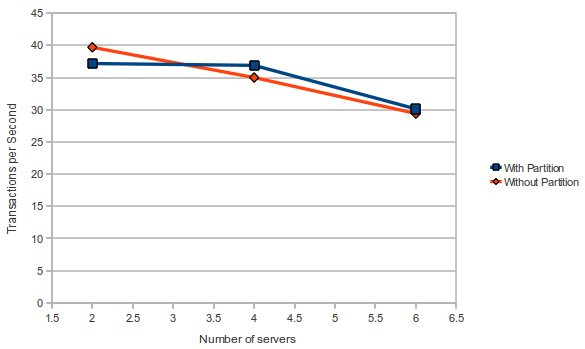
\includegraphics[scale=0.7]{peval4.png}
  \caption{Partition Test 2 -- 80 partitions}
\end{figure}

The second test also does not show a significant increase or decrease in performance. Although for 20 partitions 
the throughput did improve when re-partitioning was added in, 80 partitions did not seem to help as much. The reason
could be that the smaller range of keys were still too big such that with 80 partitions, the re-partitioning
overhead dominated the benefits.

All in all, re-partitioning does not help significantly with throughput. It seems to perform the best when 
the transactions' access range is not significantly greater than the partition's range. However, it can have
a worse effect if the partitions are too fine. Fine partitions do not work well because of the current algorithm.
Its simplicity makes it work better in the case of larger partitions. With a more sophisticated algorithm,
it would make sense for fine partitions to work well. Of course, it goes without saying that transactions that
access random uniformly distributed data will not see any improvement in throughput. In this case, it also
did not see much of a performance degradation.

\subsection{Deadlock detection}
Our deadlock detection scheme can detect deadlocks fairly efficiently. If there are two deadlocked transactions on two threads, this can be detected by one of the transactions in a time range between 8 and 100 ms. This time is measured from the start of the locking phase until the deadlock is discovered in a probe message. We tested this by setting up two transactions that tried to lock a resource held by the other at the same time. Due to concurrency issues, this test had to be repeated until a deadlock occurred. If one transaction gained both locks first, there would be no deadlock; instead, the second transaction would wait for the first to complete.

The detection time should scale with the number of deadlocked transactions because only deadlocked transactions communicate with each other. Compared to timeout-based methods, this can be quicker and more reliable than setting an upper bound on the time spent trying to acquire a lock. In this case, it might be waiting for a transaction to complete although it's not deadlocked.

The deadlock detector runs in a separate thread from each transaction's main thread, so this can cause a performance overhead. To measure the impact of the additional resources required for deadlock detection, we ran tests similar to those above with deadlock detection enabled and disabled, and we measured the transaction throughput. In these tests, we assumed that no deadlocks were present. We measured this value for 20 and 80 partitions, with the number of keys from 0 to 4000. In every case, the number of transactions per second was reduced by 15\% with deadlocking enabled, compared to deadlocking disabled. This performance overhead could be significant in a large-scale system.

These threads are always running when a transaction is occurring, and the threads are only utilized when a possible deadlock is happening. The number of probes from an origin is no more than the number of edges in the WFG, but there may be more probes from an origin if the deadlocks are not processed in a timely manner. We did not have a specific time requirement for deadlock detection and resolution, so deadlocks might not be resolved immediately if the process obtaining a lock is still running. We set a timeout to stop the process from trying to obtain a lock and to proceed with the abort if there is in fact a detected deadlock.


\iffalse
Uniform distribution of keys:

20 partitions, 4 threads, 4000 keys; re-partitioning sleeps for 5 seconds; 1200 transactions total

1 machine:
Total TPS: 3327.7499051300097

2 machines:
yes par: Total TPS: 38.21019796642812
no par: Total TPS: 38.060192839969815

4 machines:
yes par: Total TPS: 35.254050893555075
no par: Total TPS: 34.04016002821602

6 machines:
yes par: Total TPS: 29.402536313413563
no par: Total TPS: 28.96568315101926

%8 machines:
%yes par: Total TPS: 24.515095597585976
%no par: Total TPS: 22.54833324028209

80 partitions, 4 threads, 4000 keys; re-partitioning sleeps for 5 seconds; 1200 transactions total

2 machines:
yes par: Total Total TPS: 36.99719591919442
no par: Total TPS: 36.14329578690912

4 machines:
yes par: Total TPS: 34.70860934996866
no par: Total TPS: 37.0490862003126

6 machines:
yes par: Total TPS: 29.641588176339773
no par: Total TPS: 29.91988314667165

Smaller key partitioning, 20 partitions, 4 threads, 4000 keys; 5 second sleep, 1200 txns
2 machines:
yes par: Total TPS: 37.47209308960059
no par: Total TPS: 37.2844507754791

4 machines:
yes par: Total TPS: 35.73265120588351
no par: Total TPS: 34.97919960743945

6 machines:
yes par: Total TPS: 31.307083786712987
no par: Total TPS: 29.435936593733896

8 machines:
yes par: Total TPS: 23.80654480871441
no par: Total TPS: 23.19255322705625

80 partitions:
2 machines:
yes par: Total TPS: 37.199258862500415
no par: Total TPS: 39.710519111556735 

4 machines:
yes par: Total TPS: 36.90835800845145
no par: Total TPS: 35.019810606907946

6 machines:
yes par: Total TPS: 30.139539684430922
no par: Total TPS: 29.423631777261015

8 machines:
yes par: Total TPS: 24.060607266489672
no par: Total TPS: 22.690909664403264

Even smaller key partitioning, 80 partitions, 4 threads, 4000 keys; 5 second sleep, 1200 txns

6 machines:
no par: Total TPS: 27.90082070515909
yes par: Total TPS: 29.441543379468136

8 machines:
no par: 
Total TPS: 21.972720045990204
Total TPS: 21.619292443193743
yes par: 
Total TPS: 24.118879651555243
Total TPS: 22.361452467945956

Small key partitioning, 80 partitions, 4 threads, 2000 keys, 5 sec sleep, 800 txns total

\fi

\section{Future Work}

Clearly, this project is just the beginning of a much bigger project. Many questions are still left unanswered. 

Currently, two-phase commit does not have recovery process built into it. This means that the database will not
endure any kind of temporary machine failure. Future work would be to add the recovery process and logging into
the database.

The database does not support complex queries such as joins and scans. This would be supported in the future.
For a distributed key-value store, range scans are probably more important than actual database joins.

Re-partitioning is a very interesting problem. There are many algorithms for dynamically finding the best
partitioning scheme. It is not clear whether it is important to know the global state of the relationship
between partitions, or if a mere local state will be sufficient. Knowing global state would require a master
to gather all of the information. It has the advantage of being very accurate, but the disadvantage of being 
rather slow.
Local states, on the other hand, can perform ad-hoc partition transfers based on
what a few servers think are the closely related partitions. The performance should be a lot faster.
It is not clear whether local reconfigurations
will cause the system to be very inaccurate. Even with a global set of information, the transactions' profiles
may still change in such a way so that the global set is inaccurate. Future work in this area includes exploring better
algorithms for global repartitioning, and find ways to repartition distributedly.

Further optimizations for deadlock detection include localized deadlock detection and reduced probe frequency. That is, if the transactions in a WFG reside in the same server, the probing would not need to occur over RPC because the WFG would be local. This could save some RPC communication overhead in the real world, and because our database repartitions data according to how often values are accessed at the same time, this could present an opportunity to implement localized detection. The probe frequency could also be decreased following some optimizations provided by Chandy et al, perhaps by probing at certain time intervals.


\section{Conclusion}
We implemented a distributed database that supports repartitioning and deadlock detection. The database is implemented using a key-value store with tables, and it supports two-phase locking and two-phase commit. When repartitioning occurs, the heaviest-weighted partition pairs, weighted by the number of commits occurring between two partitions, are moved to the same server. The database utilizes two-phase locking and two-phase commit for each transaction. Deadlock detection is achieved by implementing a probing scheme to check for a cycle in the locking WFG, and transactions are aborted under a deadlock.

\section{References}
[1]
K. Chandy et al., "Distributed deadlock detection," ACM Transactions on Computer Systems (TOCS) 1, no. 2, 1983.

[2]
S. Ghandeharizadeh and D. DeWitt, "Hybrid-Range Partitioning Strategy: A New Declustering Strategy for Multiprocessor Database Machines," in Proceedings of the 16th International Conference on Very Large Data Bases, 1990.

[3]
C. Liu and H. Chen, "A hash partition strategy for distributed query processing," in Advances in Database Technology, 1996.

[4]
D. Mitchell and M. J. Merritt, "A distributed algorithm for deadlock detection and resolution," in Proceedings of the third annual ACM symposium on Principles of distributed computing, 1984.

[5]
C. T. Yu et al., "Partition strategy for distributed query processing in fast local networks," in IEEE Transactions on Software Engineering, 1989.



\begin{comment}

%%%%%%%%%% BIBLIOGRAPHY %%%%%%%%%%

\chapter*{Bibliography}

%

\begin{description}

\item Author, I. (Year). \emph{Book Title}, Publisher; Place of publication.

\item Lamport, L. (1986), \emph{\LaTeX: A Document Preparation System}, Addison-Wesley; Reading, MA.

\item Author, I. (Year). `Journal article title', \emph{Journal}, \textbf{Vol}, pp.first--last.

\item Smith, A.D.A.C. and Wand, M.P. (2008). `Streamlined variance calculations for semiparametric

mixed models', \emph{Statistics in Medicine}, \textbf{27}, pp.435--48.

\end{description}

\end{comment}

\end{document}

